\chapter{Programmable Computer Networks}\label{sec:ch-networks}\label{chap:nets}
Computer networks serve the important function of allowing any two machines to communicate with one another, typically via individual messages know as packets (i.e., a packet-switched network).
Naturally, reality is much more complex than this broad statement would otherwise let on; the local routing fabric in a modern network comprises specialised (though commonplace) hardware for correctly routing these packets through arbitrary topologies of links and switches at ever-increasing data rates.
This grows more complicated still when we consider the task of \emph{inter}networking between such networks, where we must route packets on higher-level logically structured addresses between different domains of control according to fairly complex policies and relationships.
At the inception of these technologies, computer scientists of the day wisely decided that the sole duty of the network itself should be the correct routing of individual packets.
Their view was that application-level logic should be executed solely at endpoint machines; their definition extended, of course, to even include desirable (and some would say indispensable) transport-level properties such as error checking and stream reliability.
This is known as the \emph{end-to-end principle}~\parencite{DBLP:journals/tocs/SaltzerRC84}.
This position arose partly due to the logical complexity of all the tasks pushed onto the network at this time, as well as the need to ensure optimal forwarding performance while microprocessors were still relatively nascent, but was instrumental in ensuring that the network itself remained \emph{extensible}.
A consistent, pared down feature set ensured while offering a good degree of freedom for the development and deployment of higher-level protocols.

Decades have passed since then, and to a large extent the zeitgeist has shifted on just how capable our networks should be---in both the research community and operators of large-scale networks.
Consider the case where an operator has a fully converged network built entirely on fixed-function hardware, but wishes to use some program to inspect the behaviour, state, and characteristics of some flow between two local machines.
The problem is that these devices offer no means of modifying or influencing routing state, being highly-optimised switching devices that understand a selection of routing algorithms built into their internal circuitry.
For the longest time, altering the network's routing behaviour in this instance---even for a single override---required not only physically altering and rewiring the network, but also would require additional hardware.\sidenote{Revisit this later... maybe a better example will come to me?}
\gls{acr:sdn} was a key development in enabling this fine-grained routing over traffic at various layers in the protocol stack, allowing operators to offer per-flow or per-class routing for improved performance---\gls{acr:te}---or even application-aware load balancers at the switch level.
Initial forays into \gls{acr:sdn} were built on the exploiting a separate \emph{control plane}, which would install \glspl{acr:mat} on target switches---mapping fields of predefined protocols to predefined actions---leaving truly complex decisions to one or more controller machines.
These developments have been pushed even further as the runtime capabilities of supporting devices have evolved into what we might now consider truly \glsxtrfullpl{acr:pdp}.
A wide variety of \glspl{acr:asic}-based switches, SmartNICs, and other accelerators now offer an environment for truly arbitrary network logic, protocol parsers, and action definitions.

Despite all this, our general-purpose Internet remains much the same from an endpoint perspective, performance and reliability increases aside.
Yet this increase in capabilities has revealed new strands of research in more specialised networks such as those in datacentres, where in-controller processing would have allowed the network fabric to \emph{cooperate} with its hosted applications but presented an obvious computational bottleneck.
\emph{In-network compute} is enabled by such bespoke routing environments such as theirs when combined with the above advances in programmability.
In-network compute is founded on the growing idea that in-path network elements such as switches, \glspl{acr:nic}s, and middleboxes can and should act as the site of complex logic to accelerate applications, participate in flow control, or to aid in network management.
%In this field
%
%?? Talk about application benefits.
%?? In-network compute.
%
%Of course, over the last 
%?? Levels of engineering work at many levels of abstraction which interlink, interlock, and depend on one another
%
%What we have now are a wide variety of ways to run programs of varying levels of complexity at ?? many levels of the stack ?? to aid application and networkr performance

In this chapter, I'll...
\section{From Fixed-Function to Fully-Programmable}

?? What are networks?

?? Possibly discuss the internet

?? Lead in from ARPAnet et al. (2 paras). Scientific comms -> general use,

The intro of choice~\parencite{DBLP:journals/ccr/FeamsterRZ14}

?? interconnection physical and reconfig are main challenges that made SDN look attractive, reasonable?

\section{Offloading in In-Network Compute}

\gls{acr:ebpf}, \gls{acr:xdp}~\parencite{DBLP:conf/conext/Hoiland-Jorgensen18}

?? mention BPFabric~\parencite{DBLP:conf/ancs/JouetP17} somewhere.

later netmap~\parencite{DBLP:conf/usenix/Rizzo12}

\section{Operation and Management}

?? network-network comms? BGP

?? IGP?

?? packets routed on a per-hop basis from their perspective: may be higher level in practice (MPLS, path switching within a gateway)

?? How can we examine this? High-level (above), mid-level ()

?? Two axes: end-to-end protocol and fabric behaviour. interact in a very delicate way (i.e., host )

?? named-data networking as potential structure of the Internet?~\parencite{DBLP:journals/ccr/0001ABJcCPWZ14}
?? Can I use this to suggest/outline problems which might be solved/encountered in a future Internet?

?? Talk about \gls{acr:as} families here: \glspl{acr:isp}, hypergiants~\parencite{DBLP:conf/sigcomm/GigisCMNKDKS21}...
?? Data centres: refer to e.g. google Espresso [sigcomm 2017] as big SDN deployments

\subsection{Fixed-Function Hardware}

\subsection{Software-Defined Networking}

?? Run through the historical context. Why? What led into P4 (OpenFlow, network operating systems...)

?? \gls{acr:ovs}~\parencite{DBLP:conf/nsdi/PfaffPKJZRGWSSA15} huge here.

?? A survey to mine for stuff~\parencite{DBLP:journals/comsur/NunesMNOT14}

?? Tie into PDP here: active networking and TPP . Think about the concept of protocol boosters~\parencite{DBLP:journals/jsac/FeldmeierMSBMR98}. (NOT READ)

\section{Traffic Characteristics}

?? Can (and should probably) discuss different traffic classes here: congestion-aware, -unaware...

?? Note, explain that this is NOT just TCP vs UDP due to existence of SCTP over UDP (See: DTLS in WebRTC), QUIC over UDP, ...

?? Chain this into \glspl{acr:cca}

?? Explain why you need what.

?? Historical context for their inclusion?

?? Discussion of evolution of traffic: what's come before, what's coming next.
?? Look for older in my old notes, but recent cite here~\parencite{DBLP:conf/anrw/BauerJHBC21}.

?? Describe all my CAIDA analysis here
?? analysis of CAIDA datasets~\parencite{caida-2018-passive}
?? congestion-aware traffic makes up at least \qtyrange{73}{82}{\percent} of packets\sidenote{\url{https://github.com/FelixMcFelix/caida-stats}}
?? Also talk about QUIC's prevalence here

\subsection{Evolution}

\subsection{Emerging Protocols}

?? QUIC~\parencite{DBLP:conf/sigcomm/LangleyRWVKZYKS17}

?? QUIC carries \gls{acr:http} traffic, mostly...

\subsection{Limitations}

\section{Problems in Modern Networks}\label{sec:problems-in-modern-networks}

\subsection{Denial of Service Attacks}
---
?? Normal ones? TCP exhaustion? Application-Level? Sheer bandwidth?

Mirai used as DDoS vector \cite{DBLP:conf/uss/AntonakakisABBB17}.

%?? Big survey \cite{DBLP:conf/imc/JonkerKKRSD17}?
\Textcite{DBLP:conf/imc/JonkerKKRSD17} offer an in-depth analysis and taxonomy of the current landscape of DoS attacks.
They observe that Denial-of-Service is most commonly achieved through \emph{resource exhaustion}---either at the target server or the infrastructure serving it.
Attacks may be classified according to two orthogonal axes: \emph{Direct vs.\ Reflection} and \emph{Volumetric vs.\ Semantic}.
\begin{description}
	\item[Direct] Attackers send packets directly towards their target. Random IP spoofing is often used to make blacklisting more difficult, but leaves evidence of an attack and its characteristics due to \emph{backscatter}, visible to internet telescopes.
	\item[Reflection] Attackers send traffic to a \emph{reflector}, spoofing the source IP of packets to match that of the target. The reflector sends replies to the target, often \emph{amplifying} them in the process.
	\item[Volumetric] DoS is achieved by \emph{resource exhaustion}---CPU or RAM usage at the target host, overfilling transmission buffers along key traffic routes. These are ``service agnostic''.
	\item[Semantic] DoS is achieved by \emph{exploiting program logic}, for instance to crash a target application server. Often tailor-made for a particular service or its deployment environment, such as \emph{Teardrop attacks}.
\end{description}
They find that TCP tends to be the leading transport for direct random-spoofing attacks, while reflection and amplification attacks are dominated by UDP-like protocols (NTP$>$DNS$>$CharGen).
Randomly spoofed direct attacks are found to last longer, and are most intense around ``web ports'' (HTTP, SSH, etc.), evidence is seen to support the existence of ``joint attacks''.
The scale of all attacks is immense, by their measurements: at least a third of the internet is under attack at any one point in time, with at least \num{30000} attacks \emph{visible} each day.

\paragraph{Amplification attacks}
abuse network services with small request bodies and large responses, causing a typically benign service to forward traffic on an attacker's behalf by \emph{reflection}---spoofing the source IP of requests to that of the intended victim.
An attacker requires that the Autonomous System (AS) they belong to doesn't prevent IP spoofing at egress.
In exchange, they are able to split their upstream bandwidth across many reflectors to gain higher volumes of attack traffic from multiple sources without revealing their own IP to the victim.

UDP-based protocols are the typical basis for such attacks, as the transport is connectionless.
While DNS is the most well-known vector for amplification, \textcite{DBLP:conf/ndss/Rossow14} presents an in-depth survey of a wide variety of other vulnerable protocols alongside a rough census of abusable servers.
He examines network services (SNMPv2, NTP, DNS, NetBIOS, SSDP), legacy services (CharGen, QoTD), peer-to-peer networks (BitTorrent, Kad), online games (Steam, Quake 3) and externally abusable botnets (ZAv2, Sality, Gameover).
Scanning for \num{e5} amplifiers of a popular service can be done in minutes, making NTP particularly dangerous due to its high amplification rate.
Furthermore, he notes that the security-focused DNSSEC can exacerbate the problem by the addition of large signatures to message payloads.

\textcite{DBLP:conf/uss/KuhrerHRH14} build further upon this census; they find significant overlap between servers who expose different vulnerable services, connect these services to OS fingerprints, and are able to use DNS proxies to enumerate the ASs who allow IP spoofing.
They find that many eligible reflectors (for i.e., DNS) tend to lie behind dynamic IP addresses and so undergo significant churn (meaning an attacker must often re-scan every few days/weeks).
This is not the case for certain protocols like NTP, where the server list remains far more stable.
The authors also explore the amplification potential of all TCP-based services---given that well-known protocols like HTTP cannot be blocked in most infrastructures, an attacker can abuse retransmissions of the handshake (\texttt{SYN-ACK}) to achieve an amplification factor up to \num{20} if the receiver doesn't send \texttt{RST}.
Differing TCP stacks have varying quirks, so the behaviour of the victim and all reflectors can be hard to predict without prior fingerprinting.
It can be observed that choosing amplifiers of larger geographic distance might increase the amount of \texttt{SYN-ACK} packets in flight before the well-meaning reflector can receive a \texttt{RST}.

NTP quickly became the attack vector of choice \cite{DBLP:conf/imc/CzyzKGPBK14}.
They find that most vulnerable amplifiers are \emph{end-hosts}, typically offering \qty{4}{\times} amplification.
At the time of publication, they observed that NTP amplification attacks had risen in volume by $\sim$\qty{1000}{\times}, though were slowly declining; of particular interest is that \qty{85}{\percent} of attacks over \qty{100}{\giga\bit\per\second} relied upon NTP reflection.
The decrease, they posit, stems mostly from vulnerable servers being patched in response to recent bulletins making the risk very clear to server operators.
How are these patched servers distributed?
They observe that, after the patch period, many of the remaining vulnerable servers are sparsely distributed (rather, the patched servers are clustered under IP blocks).
This is in line with the (un)cleanliness hypothesis put forth by \textcite{DBLP:conf/imc/CollinsSFJWSK07}.
While there were many almost comical findings (a surfeit of NTP servers holding the incorrect time, old versions), of greatest concern was the presence of ``mega-amplifiers'' offering \SIrange{e3}{e9}{\times} amplification due to the presence of network loops.
Over the duration of their study, they observed a \SI{92}{\percent} reduction in abusable IPs, though the uncleanliness observation recurs as the reduction is smaller when considering /24 prefixes (\SI{72}{\percent}).
Regardless, this drop is \emph{far} more significant than any seen in the availability of Open DNS resolvers.
A large part of the remaining vulnerable machines are identified as end hosts, implying that quick fixes are unlikely.
They make it clear that it is hard to reason about who the attackers are (bots, organisers or botmasters), and for what reasons they launch attacks (although ancillary evidence suggests that a remarkably common motivation me be rivalry through, e.g., games).

\Textcite{DBLP:conf/imc/KuhrerHBRH15} investigate the landscape of \emph{open recursive DNS resolvers}, one of the major enabling factors for DNS amplification attacks.
Specifically, a DNS server is said to be \emph{open} if it does not filter requests by source IP address.
The existence of such servers is, they claim, paradoxical: rare is the need to publicly expose recursive DNS resolution when the servers should operate in a well-structured (hierarchical) manner.
By scanning across all IPv4 addresses (according to the methodology of \textcite{DBLP:conf/uss/DurumericWH13}), they discover a downward trend in abusable servers (from \num{26.8e6} to \num{17.8e6} over the year) due to blocked requests/DNS filtering/shutdown/IP churn.
As it turns out, many of these DNS servers run old and vulnerable software, and are very highly represented (\SI{67}{\percent}) by consumer routers linked to dynamic IPs.
Curiously, cache snooping reveals that \SI{61}{\percent} of all open DNS resolvers see active use---many of these resolvers are legit (\SIrange{85}{92}{\percent}), with some even filtering out malicious domains.
The illegitimate set corresponded to censorship in Iran and China, and to malicious redirection to snooping proxies or outright malware.

As of \citeyear{DBLP:conf/imc/JonkerKKRSD17}, the distribution of amplification attacks over UDP protocols was observed to roughly have the pattern (NTP$>$DNS$>$CharGen).
This is in spite of the evidence put forth by \textcite{DBLP:conf/imc/CzyzKGPBK14}, which suggested a decline of NTP-based amplification attacks.
Perhaps the effort to patch up many servers simply hit a (metaphorical) wall of operators who actually cared, thus leaving many viable NTP amplifiers in the wild?

?? Any observations from \textcite{DBLP:conf/raid/KramerKMNKYR15}?

\paragraph{Transit-link attacks}
do some stuff according to these guys \cite{DBLP:conf/sp/SmithS18} (who defend against it), and these guys (who predicted it)---Crossfire \cite{DBLP:conf/sp/KangLG13}, Coremelt \cite{DBLP:conf/esorics/StuderP09}.

\paragraph{Characteristics}

?? Botnet C\&C communication \cite{DBLP:conf/sac/ZandVYK14}? NOT READ

?? \SI{69}{\percent} of targets are web servers \cite{DBLP:conf/imc/JonkerKKRSD17}.

DDoS attacks evolve over timescales of seconds to months.
\Textcite{DBLP:conf/spw/KangGS16} investigate this, and consider the implications and considerations necessary to deal with such occurrences.
Why might attackers desire this?
The authors posit that a diverse attack portfolio makes for more effective attacks, so long as there is \emph{variation}---a single suite or pattern of evolution makes defence (and discovery of the attacker) far simpler.
We see such evolution in:
\begin{description}
	\item[Volume and Capabilities] Peak \SI{300}{\gibi\bit\per\second}$\rightarrow$\SI{600}{\gibi\bit\per\second} over the last 4 years from date of publication.
	\item[Attack targets] E.g., Spamhaus---attackers moved from targeting endpoint servers to targeting the routers in \emph{internet exchange points} (IXPs) once the former was detected.
	\item[Strategy] E.g., semantic attacks $\rightarrow$ volumetric (TCP \texttt{SYN} flood) $\rightarrow$ volumetric (NTP amplification) $\rightarrow$ LFA.
\end{description}
They find that evolution in capabilities occurs over longer timescales, as these typically require resource acquisition (knowledge, bots, etc.).
\emph{Strategies}, however, are easily poised to evolve over short time horizons, typically ``[adapting] to the target's (observed) defensive posture''.
This behaviour was observed in both the cases of SpamHaus and ProtonMail.
In light of this, they suggest a two-tier approach to defence.
To thwart rational adversaries, they suggest the use of \emph{deterrents}---mechanisms located at e.g., a single network point, which can detect attacks and thus increase the cost of maintenance.
Most defences fit this description.
To handle cost-insensitive attackers, they suggest collaborative approaches (such as SENSS \cite{DBLP:conf/acsac/RamanathanMYZ18}).
Unfortunately, the work makes little attempt to describe or study the patterns of short-term evolution which might be expected in a real-world attack.

?? I think we need some other sources to reason about things from a game theoretic perspective---it seems to me that evolution is the name of the game \cite{DBLP:conf/atal/SinhaKT16} (not read this, but seemed relevant at the time).

\paragraph{Amplification}
\textcite{DBLP:conf/ndss/Rossow14}.
?? Inbound/outbound traffic ratios at victim (above a certain bw thres).
?? At the amp, scan activity in surrounding darknets can be an indicator.
?? At the amp, similar ratio analysis (scaled to account for benign activity and real clients who require high bandwidth: lower amp, higher bw).

\textcite{DBLP:conf/imc/CzyzKGPBK14} observe some further hallmarks specific to NTP attacks.
The \texttt{monlist} command principally used as the basis for such attacks can often reveal the list of recent targets after the fact, offering external investigators a means to determine which open NTP servers see active use as amplifiers (and their unwilling victims).
An interesting observation stemming from these records is that the sets of amplifiers and victims are both highly clustered across ASes---individually, that is.
Furthermore, it is observed that attackers choose a selection of target ports on the victim machine (in order of popularity): HTTP, NTP, SSH, gaming services and DNS.
Noting that many of thes services run on \emph{TCP}, it seems likely that attackers are hoping for firewalls to blindly allow through both TCP and UDP on these ports.
Their randomised scanning techniques imply that the culprits behind similar scans could be detected via network telescopes (although it is unclear whether this would reveal the bots, the organiser or the botmaster).

As an aside, the NTP \texttt{monlist} command fragments its $\sim$\SI{50}{\kibi\byte} payload into \SI{482}{\byte} chunks.

\paragraph{Countermeasures}
\textcite{DBLP:conf/ndss/Rossow14}.
?? AS-level---prevent IP spoofing by internal clients.
?? Protocol-level---harden w/ session handling (QUIC, Steam mostly, DTLS) at expense of latency, symmetry of req/resp size, rate limiting resps (limited use).
?? ISP-level---packet filtering on port, len, substring.

?? BGP magic against transit-link attacks and regular \cite{DBLP:conf/sp/SmithS18}.

According to \textcite{DBLP:conf/imc/JonkerKKRSD17}, the most-used techniques in deployment are \emph{DDoS Protection Services}.
While typically proprietary in nature, we see a split between \emph{cloud services}, \emph{in-line systems} (middleboxes) and hybrids thereof.

Cloud services (traffic scrubbers) are known to be most appropriate for handling volumetric attacks and are externally hosted, analysing and filtering out malicious traffic by having services redirect all inbound communication for processing.
The act of redirection is often made cheaper and/or feasible by the use of selective BGP advertisement or DNS modification, aided by reverse proxy or \emph{Generic Routing Encapsulation} (GRE).
Amongst these, BGP-based diversion is most effective where many hosts must be protected, and DNS works most reliably for single-host installations.

In-line systems, hosted within a service's domain of control, are most useful for handling semantic attacks as these often admit \emph{attack signatures} (since they must exploit a particular bug in the server).
Similarly, such attacks tend not to exhibit long-term characteristics that cloud scrubbers might use to aid detection, as many of these attacks present themselves as a single packet.

These authors further find that being attacked does not necessarily increase the likelihood of moving to a DPS---what is an effective indicator is the \emph{strength} of attack targeting a particular service.
To explain, around a fifth of targets already had a DPS prior to an attack, and only \SI{4}{\percent} of victims without a DPS migrate to one.

\Textcite{DBLP:conf/lcn/BragaMP10} have examined the detection of ongoing (flooding-based) DDoS attacks through \emph{self-organising maps}, making use of SDN to gather statistics effectively.
Many of their features aren't overly relevant, as their focus is not active defence or discovering \emph{which} hosts are contributing to an attack.

?? AmpPot \cite{DBLP:conf/raid/KramerKMNKYR15}

\emph{SPIFFY} \cite{DBLP:conf/ndss/KangGS16} aims to remedy transit-link attacks by observing how flows from each source respond to a sudden increase in available bandwidth.
\Citeauthor{DBLP:conf/ndss/KangGS16} realise that bots participating in an attack are often unable to match this bandwidth expansion due to having already saturated the capacity of their outbound links, while legitimate flows typically speed up to match the new fair-share rate.
%Attackers must either be detected or reduce the throughput of each bot, increasing the cost of launching an attack.
Unlike our approach (and due to the class of attacks it is designed to defend against), SPIFFY is intended to be deployed within ISP networks, although some of our feature choices are backed by similar observations.
?? Flaws? what can't it do that we can do better? Long times to compute TBE routes on real networks, low expansion factor in real network can require more ``rounds'' of filtering. (``takes only'' \SI{14}{\second} for Cogent network? gross.)
?? I believe their assumptions may not extend to CBR traffic (e.g., UDP VoIP traffic), which we know makes up a sizeable proportion of network traffic.

\emph{Athena} \cite{DBLP:conf/dsn/LeeKSPY17} is a more generalised SDN framework for intrusion detection, but has shown the use of a \emph{k-nearest neighbours} classifier to detect individual attack flows.
Although heavyweight (and proven to be effective compared with \textcite{DBLP:conf/lcn/BragaMP10}), their comparison against SPIFFY lacks the quantitative evidence required to understand how the system compares.

SENSS \cite{DBLP:conf/acsac/RamanathanMYZ18} aims to help hosts and/or \emph{endpoint-servers} communicate upstream with ISPs.
The rationale is that, although DDoS traffic can be filtered at any point along its path it will impact less of the network if it is filtered \emph{close to its source}---this observation holds true in all attack classes (direct, reflection, LFA/crossfire), which exhibit a tree-like pattern of traffic.
This information currently propagates through human channels, eventually leading to traffic black-holing being performed by key ASes.
The core idea is that the \emph{victim} should be given responsibility for intelligence and decision-making, who pass on their requests to ISPs (alongside ample payment)---they are able to show that this approach functions for multiple algorithms.
The need for payment does seem odd at the outset, but it becomes clear that this is a necessary mechanism to enable ``remote networks to collaborate on demand, without prior trust''.
While all the software engineering work seems well-considered, it appears to hinge on the condition that HTTP/TCP sessions can be reliably held over the saturation zone between high-priority endpoints---they do admit that alternative channels may be possible through elected proxies or UDP-based mechanisms like DOTS \cite{ietf-dots-use-cases-17}.
The mitigation strategies they propose do hold water, and strike me as interesting---using NAT for true outbound requests as a mechanism for reflector filtering close-to-source, similar techniques to others to ``route around'' the congestion added by LFAs, and location-based filtering for signature-free attacks.
What I'm concerned about is the degree of collaboration required; it seems likely to me that there may exist e.g., amplifiers who are difficult to block in such a manner due to non-cooperative ASes on their path, with geography and network uncleanliness as contributing factors...
Their evaluation is convincing---a mixture of a testbed experiment over a small-scale environment (Iperf + ``custom UDP flood'') and an AS-level simulation recreating the DDoS attack on Dyn (gravity model \cite{DBLP:journals/ccr/Roughan05}, cogent topology from Topology Zoo \cite{topology-zoo}).

?? Collaborative soln (?) \cite{DBLP:journals/tnsm/SimpsonSMJPH18}

\Textcite{DBLP:conf/sp/SmithS18} present techniques based on AS-level routing to tackle both transit-link and flooding-based attacks.
This view is taken due to the perceived cost of per-stream classification and inherent sensitivity to adversarial examples or crafted input.
The approach is creative, relying upon BGP \emph{fraudulent route reverse poisoning} to preserve traffic to a target AS, but unlike SPIFFY the approach doesn't actually \emph{remove} the congestion.
Because of this, traditional flooding-based attacks aren't fully alleviated.

?? DDoS Open Threat Signalling \cite{ietf-dots-use-cases-17} as an architecture to maybe enable the deployment of many of these?

\subsection{Scaling}

\subsection{Fairness}

\section{SFC Notes}
SafeBricks~\parencite{DBLP:conf/nsdi/PoddarLPR18} extends the prior NetBricks~\parencite{DBLP:conf/osdi/PandaHJWRS16} to take advantage of TEEs.
The main framework goals above the benefits of TEEs themselves are to protect traffic from the NF (i.e., inappropriate field/packet accesses) and protect NF source code from the framework.
The execution model is a directed graph of smaller user functions including branches etc., where each NF is given access to specific packet regions by a framework (attaching a permission set to each sub-NF at build time).
This executes as a single binary in the TCB/TEE because enclave swaps in/out are particularly costly (complete cache flushes, re-encryption etc.).
DPDK daemon in userland passes packets in (i.e., Scone below)---one executing pipeline (though surely could be multiple in theory?).
NF source code (and any pre-encrypted proprietary NF source codes) are given to \emph{trusted binary} which includes all details and attested in the same manner as the compiled program.

AuditBox adds \emph{verified routing protocols} (VRPs) to this~\parencite{DBLP:conf/nsdi/LiuSKPSS21}.
This enables routing packets \emph{between enclaved NFs} (i.e., explicitly separate machines), and ensuring that the right paths are being followed, the network is not altering packets, and the network is not reordering packets (preventing MITM).
Additionally, this allows path auditing in a way which is invisible to NFs and the network (i.e., print log for like \qty{1}{\percent} of packets).
Versus prior VRPs, this enables dynamic routing between NF segments (i.e., selective filtering to a lighter or heavier function based on local state).
Note that you can do this \emph{in one box} using SafeBricks, the novelty here pertains to adaptively routing \emph{between several boxes}.
Cost? Halves goodput vs. NetBricks.

\section{Programmable Data-Planes}

\begin{figure}
	\resizebox{\linewidth}{!}{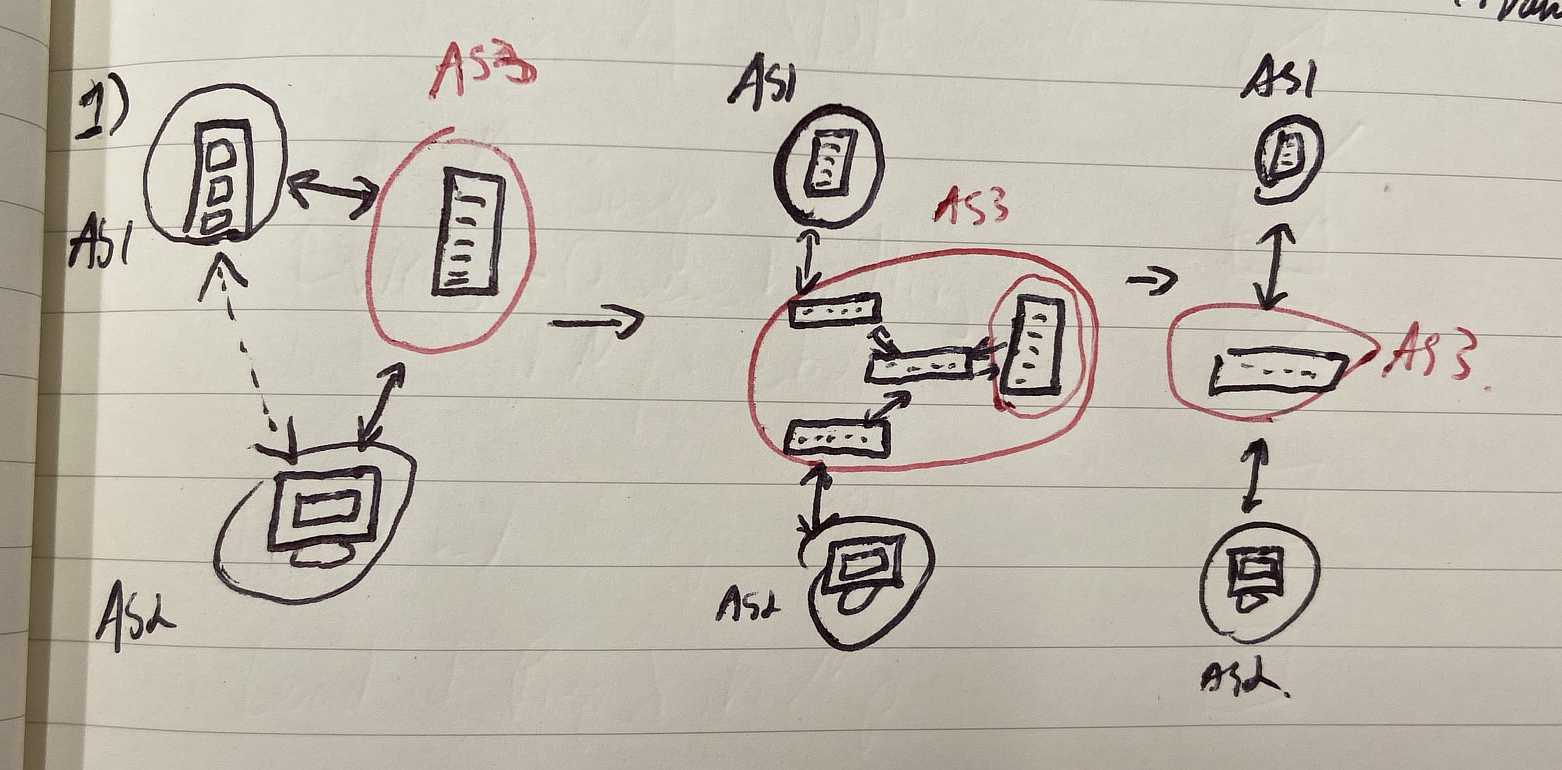
\includegraphics{diagrams/pdp-lit/steering-draft}}
	\caption{text}\label{fig:pdp-lit-steering}
\end{figure}

\begin{figure}
	\resizebox{\linewidth}{!}{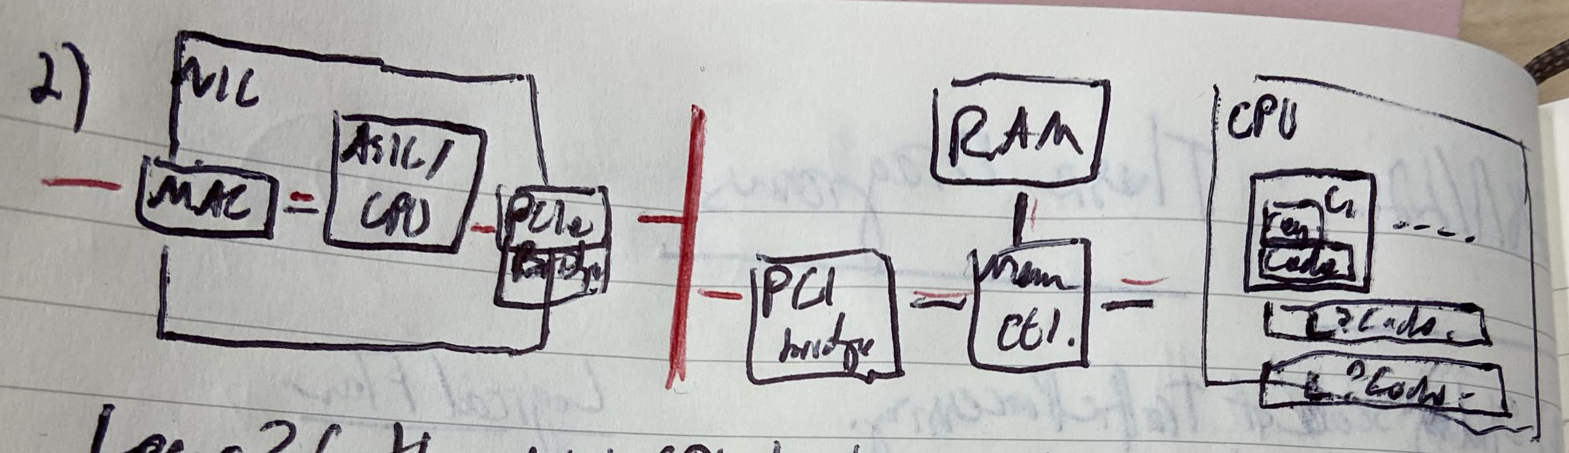
\includegraphics{diagrams/pdp-lit/pci-draft}}
	\caption{text}\label{fig:pdp-lit-pci}
\end{figure}

\begin{figure}
	\resizebox{\linewidth}{!}{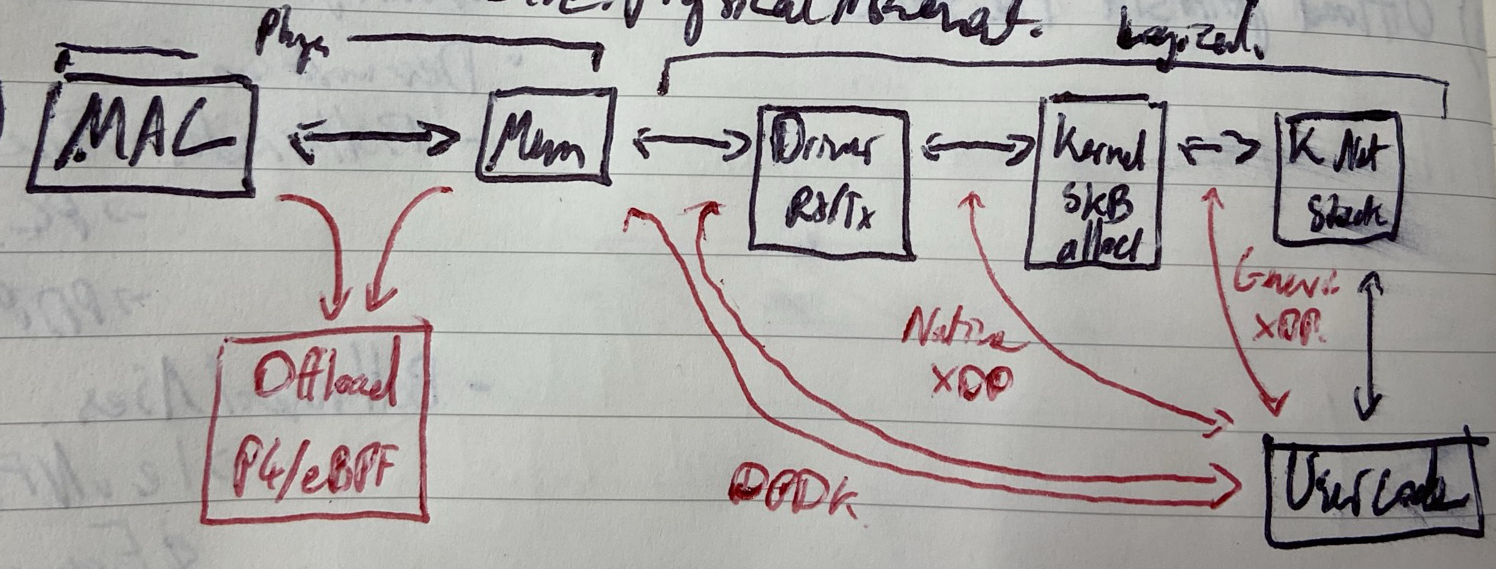
\includegraphics{diagrams/pdp-lit/offloading-draft}}
	\caption{text}\label{fig:pdp-lit-offloading}
\end{figure}

?? 2021 --- crucial to sell the why! What can be gained moving to this level, new state measures enable new applications, in-nic/switch exec reduces latencies, increases throughputs, etc...
?? Probably want a worked example showing how in-network compute helps. I.e., network graph, show processing at nodes

?? Explain \gls{acr:npu} here...

?? Understanding Host Network Stack Overheads~\parencite{DBLP:conf/sigcomm/CaiCVH021}

?? Evidence of deployment in real, huge transit networks~\sidenote{\url{https://wiki.geant.org/display/RARE/Home}, \url{https://wiki.geant.org/display/NETDEV}}

?? arbitrarily reconfigurable hardware located directly on the data path

?? OvS?~\parencite{DBLP:conf/sigcomm/TuWAP21}

?? mention how it came to this: this was an alternate solution to latency or throughput concerns which plague VNF approaches as they scale (see Metron paper for good discussion of RSS, etc., which solve these problems in their own way)

?? new ways to implement stateful + stateless packet processing.

?? History? RMT~\parencite{DBLP:conf/sigcomm/BosshartGKVMIMH13}, ClickNP, GPU offload papers. See Metron paper for cites.

?? NetFPGA~\parencite{DBLP:conf/fpga/IbanezBMZ19}

?? Getting even faster?~\parencite{nokia-fp5}

\sidenote{Test text hello.}

?? RMT was the first big innovation over OpenFlow --- read this!!

\section{Control and Management}

?? Refer back to History through OpenFlow -- what prompted the evolution?

?? Control of these devices has a lot in common with OpenFlow -- controller, except using commodity hardware to install firmwares, and so on,

\section{Software Frameworks}

\subsection{eBPF}
?? eBPF

?? BPFabric

\subsection{P4}
?? P4

?? Others who lost?

?? How do these differ? What do they share?

?? Popular frameworks now support this -- ONOS, eBPF translators, behavioural model software switch...

?? Things like Lucid built on top of P4?~\parencite{DBLP:conf/sigcomm/SonchackLRW21}

?? P4~\parencite{DBLP:journals/ccr/BosshartDGIMRSTVVW14} and \emph{programmable dataplane} (PDP) hardware~\parencite{DBLP:journals/micro/ZilbermanACM14, netronome-smartnic, xilinx-alveo, barefoot-intel}

?? Cool NIC-CPU co-design~\parencite{DBLP:conf/osdi/IbanezMAJ0KM21}

\fakepara{PDP design for asynchronous compute}
\emph{PANIC}~\parencite{DBLP:conf/hotnets/StephensAS18} places a routing fabric between distinct packet/data processing elements \emph{in a SmartNIC}.
Such designs would enable general, asynchronous, and novel compute in SmartNICs and switches, for instance offering consistent and easy to use communication between workers versus hard-coded ME relationships.
Event-driven versions of P4 have been suggested~\parencite{DBLP:conf/hotnets/IbanezABM19}.
Timer events and device state changes would empower in-network RL use-cases, signalling timesteps for RL agents or new, effective, fine-grained sources of input state.

\section{Offloading frameworks}
\emph{ClickNP}~\parencite{DBLP:conf/sigcomm/LiTLPLXXC16} targets NetFPGAs: DAG of predefined Click-like blocks, i.e. VHDL segments.
Why?
The C$\rightarrow$VHDL pipeline leads to awful code, so this achieves better FPGA usage.

\emph{Floem}~\parencite{DBLP:conf/osdi/PhothilimthanaL18} presents a DSL in python, which compiles to C for host and specific target NIC.
This does require specific dev effort per-target-NIC.

\emph{iPipe}~\parencite{DBLP:conf/sigcomm/LiuCSKPG19} runs C language programs on SmartNIC (intended) and host (emergency) according to whether traffic is at-risk of suffering from SmartNIC resource contention.
Processing is dynamically `unoffloaded' back to the host machine if SmartNIC load is too great.
This requires identical language support on both accelerator and host---which is very much not guaranteed.

\emph{hXDP}~\parencite{DBLP:conf/osdi/BrunellaBBPSBCP20} allows eBPF execution on FPGA---supports expanded eBPF ISA rather than converting program into a complete pipelined circuit (i.e., this runs as a coprocessor).
Why?
Fast redesign/reinstall time: a complete circuit bake takes ages, while JITing and compiling an eBPF program into their new ISA is pretty fast.
This includes some very cool details on around VLIW instruction-level parallelism built into their ISA and figured out during compile-time.

\emph{Gallium}~\parencite{DBLP:conf/sigcomm/ZhangZK20} converts a C++ (ClickNF program)$\rightarrow$auto-leverage PDP (P4 + C++ + P4).
Split into pre- and post-host P4 segments, with a host C++ program.
Gallium uses LLVM IR to determine read-write dependencies between variables/basic-blocks, account for PDP capabilities of packet reads (i.e., PDP can't touch packet body past $\sim$\qty{300}{\byte}), can move about \qty{100}{\byte} metadata between sites.
Identifies fast/slow paths if offloading can be elided.
Main drawback is that some annotation needed to translate Click primitives into MATs etc., otherwise the conversion to P4 means minimal additional work per target accelerator.

\emph{Flightplan}~\parencite{DBLP:conf/nsdi/SultanaSGPHSBDL21} splits P4 program into subchunks placed and routed between \{PDP, FPGA, host, server, NPU, ASIC\} for pipelining (i.e., performance) or redundancy.
Their disaggregation inserts blocks before and after splits to handle metadata (state) passing.
Their compiler breaks the programs on basic blocks with user annotations, where specific implementations manually given for some \texttt{extern}s to enable device-specific acceleration.
Data dependencies between basic blocks are extracted from the P4 IR in P4C compiler.

Preliminary work on splitting eBPF programs between an XDP part and userland part has been proposed~\parencite{DBLP:conf/conext/ShahinfarMSSBA21}.
This considers both horizontal (i.e., chunks in driver with XDP tail-calls) or vertical (user$\leftrightarrow$kernel) splits of code.
I think their XDP vs.~AF\_XDP split test confirms that the first handler in the XDP hook is basically single-threaded, which probably has some implications for our use of it as an offload.

\paragraph{Misc P4 translations.}
T4P4S~\parencite{DBLP:conf/hpsr/VorosHKLTL18} converts P4 programs into C, which are linked against a target-specific network hardware abstraction layer.
This seems to be the most effective host deployment for P4 at the moment, since it buys you DPDK-capable P4 dataplane installation compared to how terribly slow BMv2 is known to be.
Slower than native DPDK, but outpaces OvS, and allows definition of HAL binaries in SmartNIC C code as needed too.

$\mu$P4~\parencite{DBLP:conf/sigcomm/SoniR0DF20} extends P4C to decompose parser and action code into independent subprograms, to simplify porting behaviours between different switch models (V1Model, PSA, SUME, ...).

Lyra~\parencite{DBLP:conf/sigcomm/GaoZLMZTSCZY20} is a language for running Network Programming Language friendly programs (i.e., same constraints as P4 programs) across heterogeneous switch hardware, plus placement constraints.

?? P4 Verification~\parencite{DBLP:conf/sigcomm/TianGLZCZDYMTLW21}---also shows use of \gls{acr:pdp} switches in real large-scale networks (\gls{acr:isp}?)

\section{Use Cases}

?? On-switch (Tofino) DDoS detection and defence \url{https://www.usenix.org/conference/usenixsecurity21/presentation/liu-zaoxing}

\subsection{In-Network Computation}\label{sec:in-network-computation}
?? In-network computation.\sidenote{Test text hello.}

iSwitch~\cite{DBLP:conf/isca/LiLYCSH19} uses programmable switches to combine model updates between RL agents acting as part of a distributed RL training system.
Note that we discuss this in section \ref{sec:wtf}.\sidenote{Make sure that this is properly explained in the PDP seciton: source is `report-yr2.tex'.}

?? Taurus moved out of representations section~\parencite{DBLP:journals/corr/abs-2002-08987}

?? A recent line of research in the community has been to investigate \emph{Binarised/Bitwise Neural Networks} (BNNs)~\parencite{DBLP:conf/nips/HubaraCSEB16,DBLP:journals/corr/KimS16,DBLP:journals/corr/MiyashitaLM16} for line-rate packet classification.
?? \emph{BaNaNa SPLIT} shows this as an offload mechanism~\parencite{DBLP:conf/sigcomm/SanvitoSB18,DBLP:journals/corr/abs-1801-05731}; DNN inference is often carried out on the \emph{CPU} to reduce latency imposed by GPU batching and transfer, but fully-connected layers can be accelerated further by NICs.

\subsection{Network Telemetry}
?? Others (try to avoid DDN cases here).

?? The P4 ecosystem already presents novel, openly-available, fine-grained traffic measurement techniques that can be installed and controlled with ease~\parencite{DBLP:conf/sigcomm/GuptaHCFRW18,DBLP:conf/sigcomm/ChenFKRR18,DBLP:conf/sosr/GhasemiBR17}

\subsection{Transport Layer Optimisation}
?? Hi~\parencite{DBLP:conf/nsdi/ArashlooLGRWW20} Network stacks being moved into NICs to reduce latency/CPU utilisation, mainly for datacentre use-cases---otherwise, \SI{100}{\giga\bit\per\second} can't be hit. New API \emph{Tonic} for transport layer in user code (send, data management), DMA to NIC and let it handle all (de)packetisation. ``Transport logic'' goes to Tonic. Main design is datacentres, so not very high BDPs (long-fat) $\rightarrow$ \si{\kilo\byte} inflight data.

\subsection{Active Queue Management}
Turns out that you can't just write it in P4, you need to co-design for the target environment---with meaningful performance cost to boot, based on the tradeoffs you need to make~\parencite{Kunze-P4-AQM}.

\subsection{KV Stores}
NetChain~\parencite{DBLP:conf/nsdi/JinLZFLSKS18}.

\subsection{ML in PDP}
?? ML in the dataplane~\parencite{DBLP:conf/hotnets/XiongZ19,DBLP:conf/sigcomm/SanvitoSB18,DBLP:journals/corr/abs-1801-05731,DBLP:journals/corr/abs-2009-02353,langlet-ml-netronome,DBLP:journals/corr/abs-2002-08987}

\section{Hardware Designs}

?? Mention FPGA vs many-core

?? P4 etc. can actually all run on commodity hardware, which offers a third (suboptimal) hardware class.

?? Ref the paper that Haruna presented \parencite{DBLP:conf/icc/MafiolettikDMRV20}: pareto front of work-division optimality for SmartNICs (i.e., addition of high-latency cores).

?? How do these limit and influence what code can be run on different device classes? The time taken to adapt the network?

\subsection{Models of Parallelism}

\subsection{Flexibility}

\subsection{Mapping Software Frameworks}

\section{Summary}
Eh.
